%!TEX root = ../report.tex

% Du har lavet antallet af klynger om, så skriv gerne det her om ifht. det nye antal af klynger \#todo


%%%%%%%%%%%%%%%%%%%%%%%%%%%%%%%%%%%%%%%%%%%%%%%%%%%%%%%%%%%
\chapter{Delanalyse 1: Opdeling af arbejdsmarkedet i delmarkeder \label{kapitel_delanalyse1_deskriptivt}}
%%%%%%%%%%%%%%%%%%%%%%%%%%%%%%%%%%%%%%%%%%%%%%%%%%%%%%%%%%%

Dette kapitel har til formål at svare på det første forskningsspørgsmål:

\begin{tcolorbox}[title=Forskningspørgsmål,
subtitle style={boxrule=0.4pt} ]
	\tcbsubtitle{1.} Er der en opdeling af arbejdsmarkedet for arbejdstagere i delmarkeder, hvor mobilitet indenfor delmarkederne er hyppig, og mellem delmarkederne sjælden?
\end{tcolorbox}

Dette forskningsspørgsmål vil jeg besvare ved at vise resultatet af min analyse - en opdeling af arbejdsmarkedet for arbejdstagere i delmarkeder. Spørgsmålet er såvidt der er en opdeling, om opdelingen afspejler de få delmarkeder i amerikanske regi \parencite{Piore1980, Gordon1982} eller flere små delmarkeder ligesom i dansk regi \parencite{Boje1985, Touboel2013}.

Men det i sig selv er ikke svar på forskningsspørgsmålet. For at vudere, om der er en reel opdeling af det danske arbejdsmarkede i delmarkeder, hvor mobilitet indenfor delmarkederne er hyppig, og mellem delmarkederne sjælden, så er det nødvendigt at vurdere kvaliteten af delmarkederne.

Jeg vil først vurdere kvaliteten ved at forklare dannelsen af delmarkederne med Moneca-algoritmens klyngedannelse.

Dernæst vil jeg sætte fokus på jobmobilitet, fordi det er et helt centralt begreb som forklaring af opdelingen af delmarkederne. For Boje er det helt centralt, at der er begrænset mobilitet mellem de enkelte delmarkeder. 


%%%%%%%%%%%%%%%%%%%%%%%%%%%%%%%%%%%%%%%%%%%%%%
\section{Opdeling af arbejdsmarkedet i klynger \label{delanalyse1_endelige mobilitetskort}}
%%%%%%%%%%%%%%%%%%%%%%%%%%%%%%%%%%%%%%%%%%%%%%

Analysen viser 51 klýnger på det danske arbejdsmarked. Med så mange klynger ligger resultatet sig langt fra få delmarkeder i amerikanske regi \parencite{Piore1980, Gordon1982} og tættere op imod de danske undersøgelser \parencite{Boje1985, Touboel2013}.

Klyngerne fremstår i figur \ref{fig_delanalyse1_kort_seg_proces5} som et netværk af 273 noder opdelt i de 51 klynger. De 273 noder dækker hver især over jobfunktioner. Disse jobfunktioner bindes sammen af strege, som viser mængden af jobskifte mellem forskellige jobfunktioner fra år til år. Jo flere jobskifte, der er mellem jobfunktioner, jo kraftigere er stregene. Eksempelvis er stregene kraftigere mellem snedkerarbejde og tømrerarbejder, da der i perioden 1996 til 2009 var XXXX personer, der skiftede job herimellem.

\begin{figure}[H]
\begin{centering}
  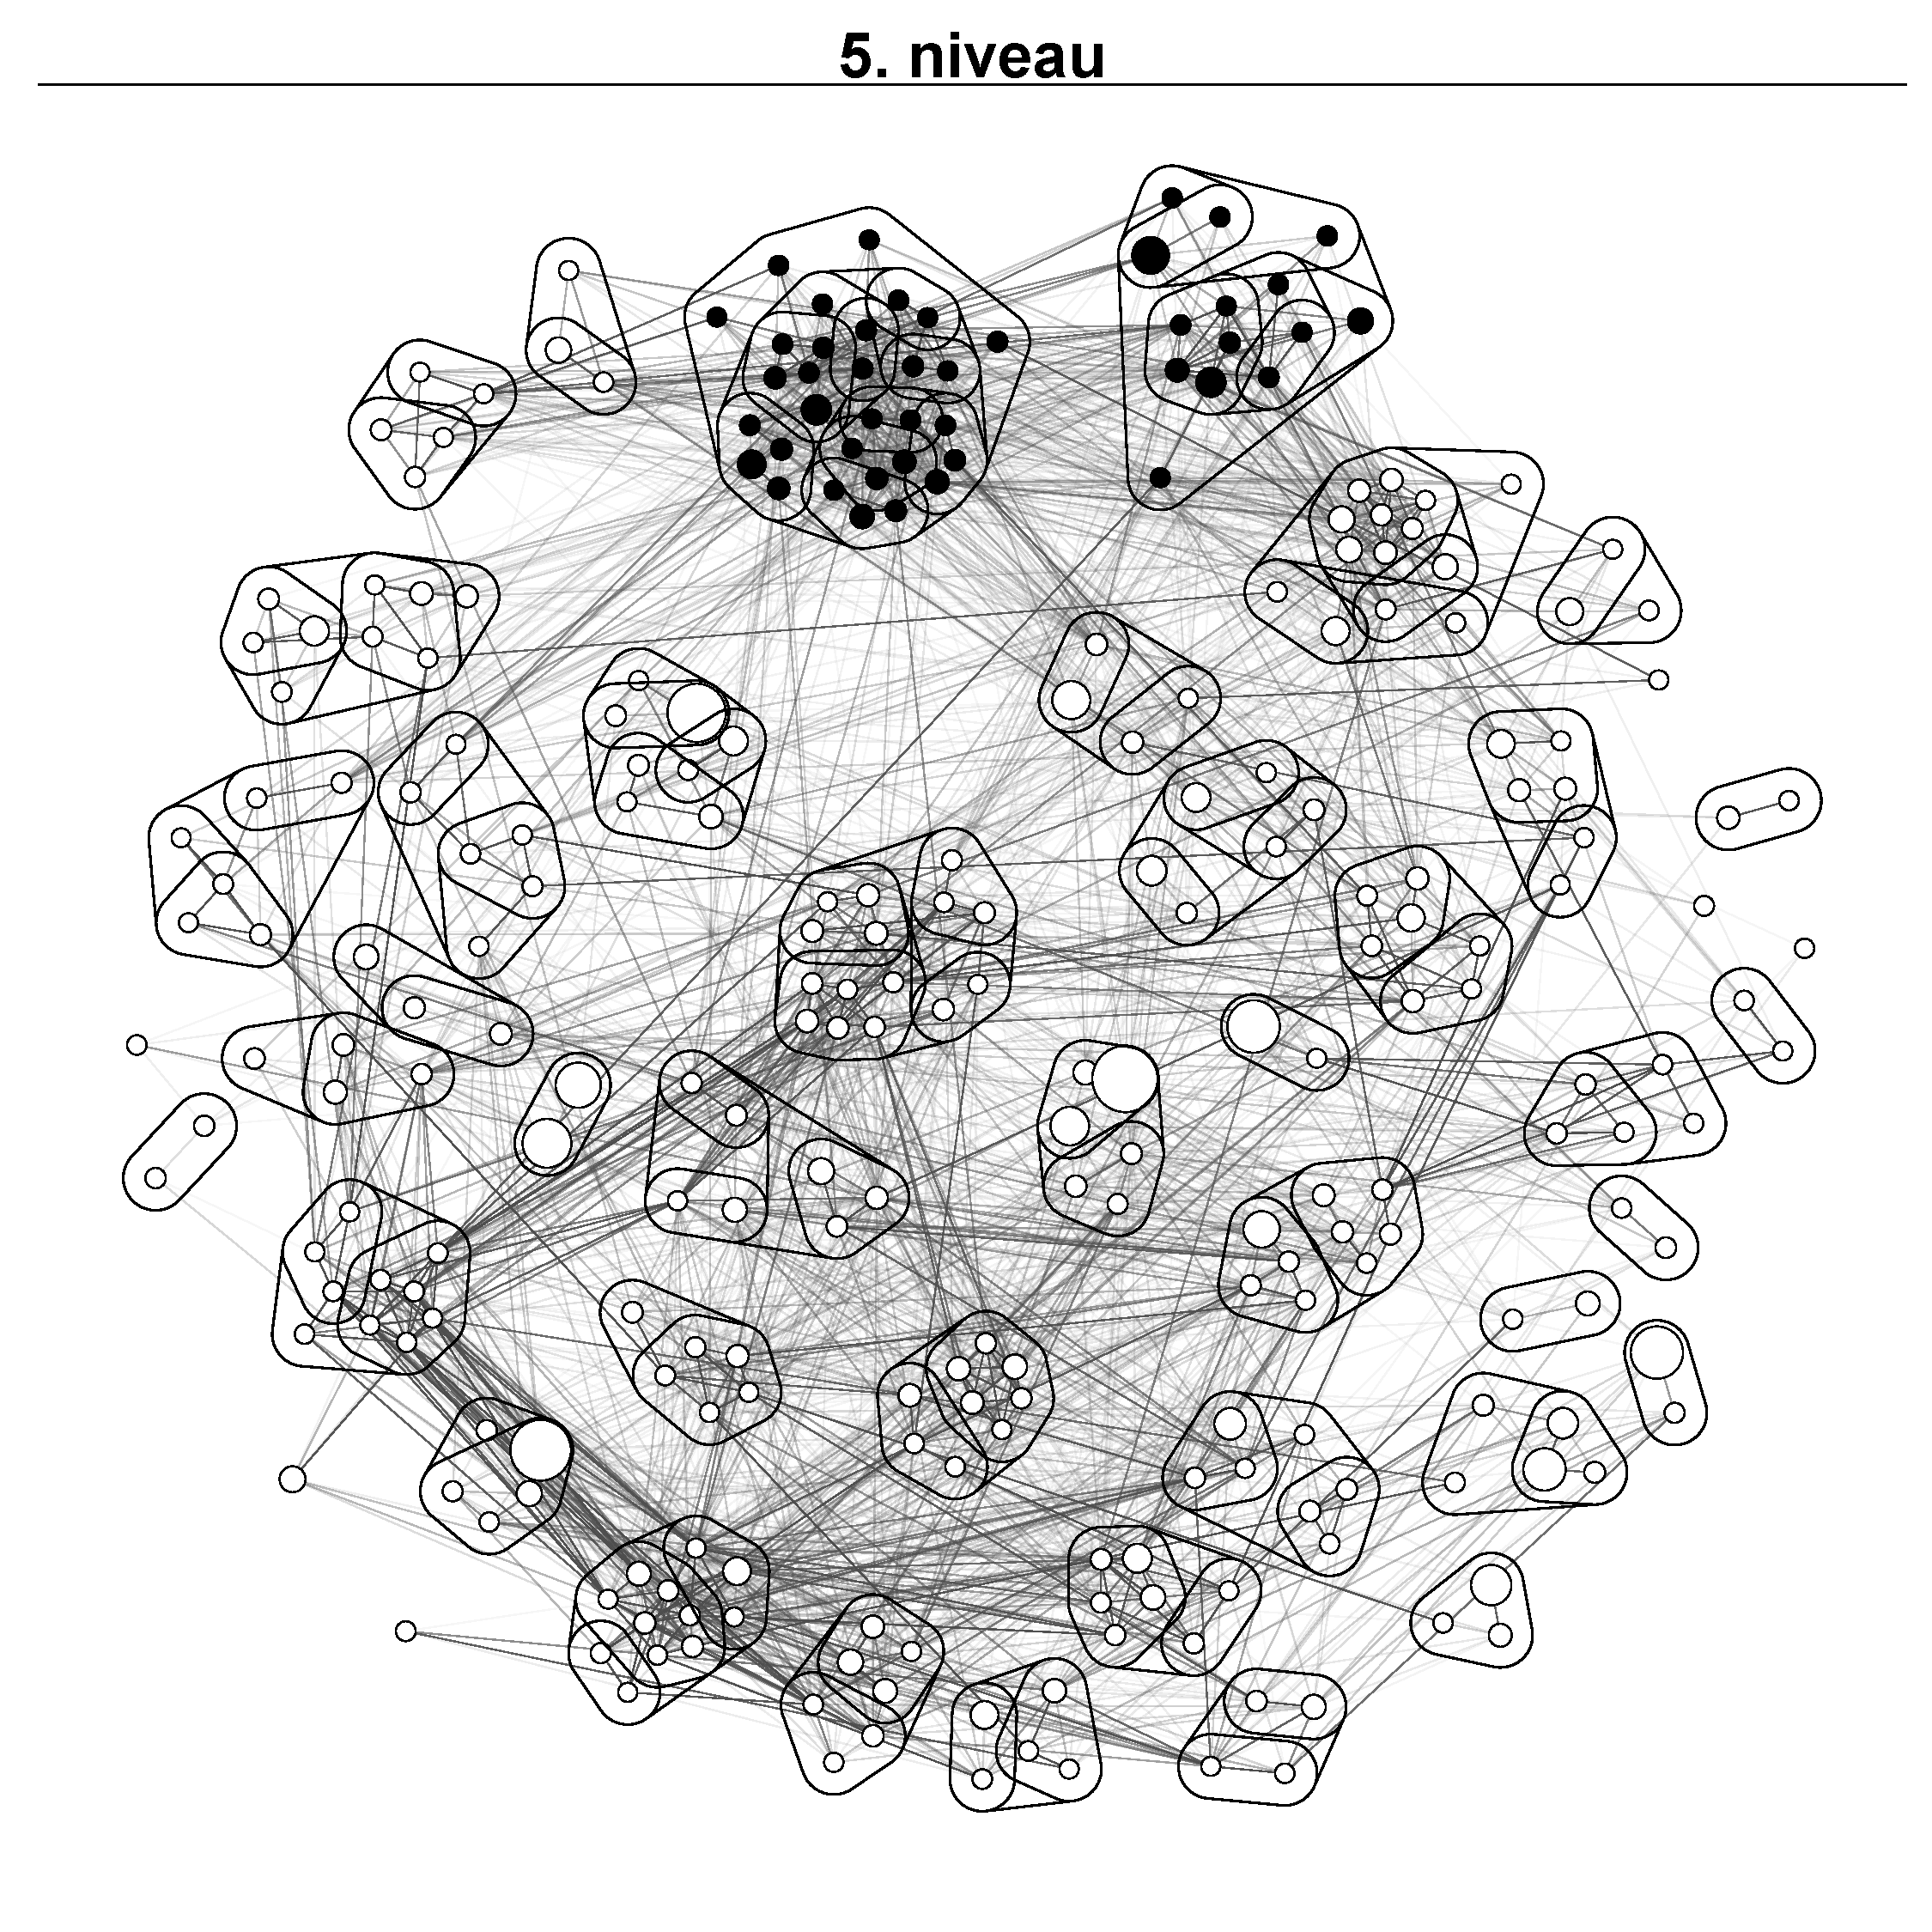
\includegraphics[width=10 cm]{fig/netvaerkskort/kort_seg_proces5.pdf}
  \label{fig_delanalyse1_kort_seg_proces5}
  \caption{}
\end{centering}
\end{figure}

Klyngerne er blevet skabt via Moneca-algoritmens klyngedannelse. Afhængigt for om klyngerne også er deciderede delmarkeder er jobmobilitet, \emph{densiteten} og \emph{den maksimale stilængde}. For at der er tale om et delmarked skal der ifølge Boje været meget mobilitet indenfor delmarkedet og barrierer for jobmobilitet mellem  delmarkeder. Derfor et jobmobilitet det mest centrale mål i dannelsen af delmarkeder. Samtidig er \emph{densiteten} og \emph{den maksimale stilængde} yderligere centrale mål i dannelsen af klynger.

Til sammen er sammenhængen mellem jobmobilitet, \emph{densiteten} og \emph{den maksimale stilængde} for en række noder med til at sige, om vi har at gøre med et delmarked eller ej. Når snedkerarbejde og tømrerarbejder er i samme klynge sammen med andet faglært arbejde har det således at gøre med, at der er mange, der skifter job imellem denne type faglært arbejde samt at der er tilstrækkelig med jobskifte mellem af jobfunktionerne i klyngen. For at parafrasere Weber, så består et delmarked af de arbejdsmarkedssituationer, hvor mobilitet er nem og typisk 
%
\footnote{Parafrasen er over citatet “\emph{A »social class« makes up the totality of those class situations within which individual and generational mobility is easy and typical.}” \parencite[302]{Weber1978}.}%
%
\parencite[302]{Weber1978}.

Dette er dog i sig selv ikke svar på, om der er en opdeling af arbejdsmarkedet for arbejdstagere i delmarkeder, hvor mobilitet indenfor delmarkederne er hyppig, og mellem delmarkederne sjælden. For at vudere, om der er en reel opdeling af det danske arbejdsmarkede i delmarkeder, så vil jeg først vurdere kvaliteten ved at forklare Moneca-algoritmens klyngedannelse. Dernæst vil jeg sætte fokus på jobmobilitet, fordi det er et helt centralt begreb som forklaring af opdelingen af delmarkederne.


%%%%%%%%%%%%%%%%%%%%%%%%%%%%%%%%%%%%%%%%%%%%%%
\section{Dannelsen af klynger \label{delanalyse1_segmenteringsprocessen}}
%%%%%%%%%%%%%%%%%%%%%%%%%%%%%%%%%%%%%%%%%%%%%%

Klyngerne er blevet skabt via Moneca-algoritmens klyngedannelse. Afhængig for klyngedannelsen er jobmobilitet, \emph{densiteten} og \emph{den maksimale stilængde}.

Klyngedannelse sker ved at aggregere erhvervskategorier i klynger, baseret på deres mobilitetsmønstre. Aggreringen af klynge sker i en række faser ind til det ikke længere. Årsagen til, at det ikke længere er muligt skyldes mangel på jobmobilit og \emph{densitet} og for lange \emph{stilængder}.

Moneca-algoritmens klyngedannelse sker således på fem niveauer. I første niveau starter vi med de 273 noder, der hver især dækker over jobfunktioner fx snedkerarbejde eller tømrerarbejde. I femte og sidste niveau er de 273 noder blevet aggreret til de 51 klynger fx klyng, hvor snederarbejde og tømrerarbejde er blevet aggreret sammen med en række andre jobs inden for faglært arbejde.

Aggreringen fra nivea 1 til niveau 5 fremgår af tabel \ref{tab_delanalyse1_karakteristika}, der viser et overblik over klyngedannelsen, med den gennemsnitlige interne og eksterne mobilitet i klyngerne, for hvert klyngedannelsessniveau.
% 
\begin{table}[H] \centering
\caption{Karakteristika for klyngedannelsen}
\label{tab_delanalyse1_karakteristika}
\resizebox{.8\textwidth}{!}{%
\begin{tabular}{@{}l|rrrrr@{}}
Niveau	&	1. niveau	&	2. niveau	&	3. niveau	&	4. niveau	&	5. niveau	\\		\midrule
Antal klynger	&	273	&	114	&	68	&	53	&	51	\\		
Reduktion i antal klynger	&	-	&	139\%	&	68\%	&	28\%	&	4\%	\\		\midrule
Intern mobilitet (gns.)	&	68\%	&	75\%	&	77\%	&	78\%	&	79\%	\\		
Ekstern mobilitet (gns.)	&	32\%	&	25\%	&	23\%	&	22\%	&	21\%	\\		\midrule
Mobilitet i alt	&	100\%	&	100\%	&	100\%	&	100\%	&	100\%	\\		
Forøgelse i intern mobilitet	&	-	&	10\%	&	3\%	&	2\%	&	1\%	\\		\midrule
\end{tabular} }
\end{table}
%
I de følgende afsnit beskrives aggreringen fra niveau til niveau med henblik på at vrdere kvaliteten af klyngerne.


%%%%%%%%%%%%%%%%%%%%%%%%%%%%%%%%%%%%%%%%%%%%%%
\subsection{Niveau 1}
%%%%%%%%%%%%%%%%%%%%%%%%%%%%%%%%%%%%%%%%%%%%%%

Niveau 1 er uaggreret med de 273 noder, der hver især dækker over jobfunktioner. Det første iøjnefaldende er at den interne mobilitet på det er højt i sig selv. 68 \% skifter altså job inden for de 273 noder. Det vil sige en tømrer skifter job fra en virksomhed til en anden. Det indikerer at en væsentlig mængde skift foregår på et meget lavt \texttt{DISCO}-niveau. Langt de fleste bliver indenfor deres eget job%
%
\footnote{Eller ihvertfald et job, der ligger så tæt på, at man selv på mit usædvanligt lave 4-cifrede \texttt{ISCO}-niveau ikke kan skelne dem fra hinanden.}%
%


%%%%%%%%%%%%%%%%%%%%%%%%%%%%%%%%%%%%%%%%%%%%%%
\newpage \subsection{Niveau 2}
%%%%%%%%%%%%%%%%%%%%%%%%%%%%%%%%%%%%%%%%%%%%%%


\begin{wrapfigure}{r}{8cm}
  \vspace{-20pt}
  \begin{center}
   \caption{}
   \label{fig_delanalyse1_kort_seg_proces2}
    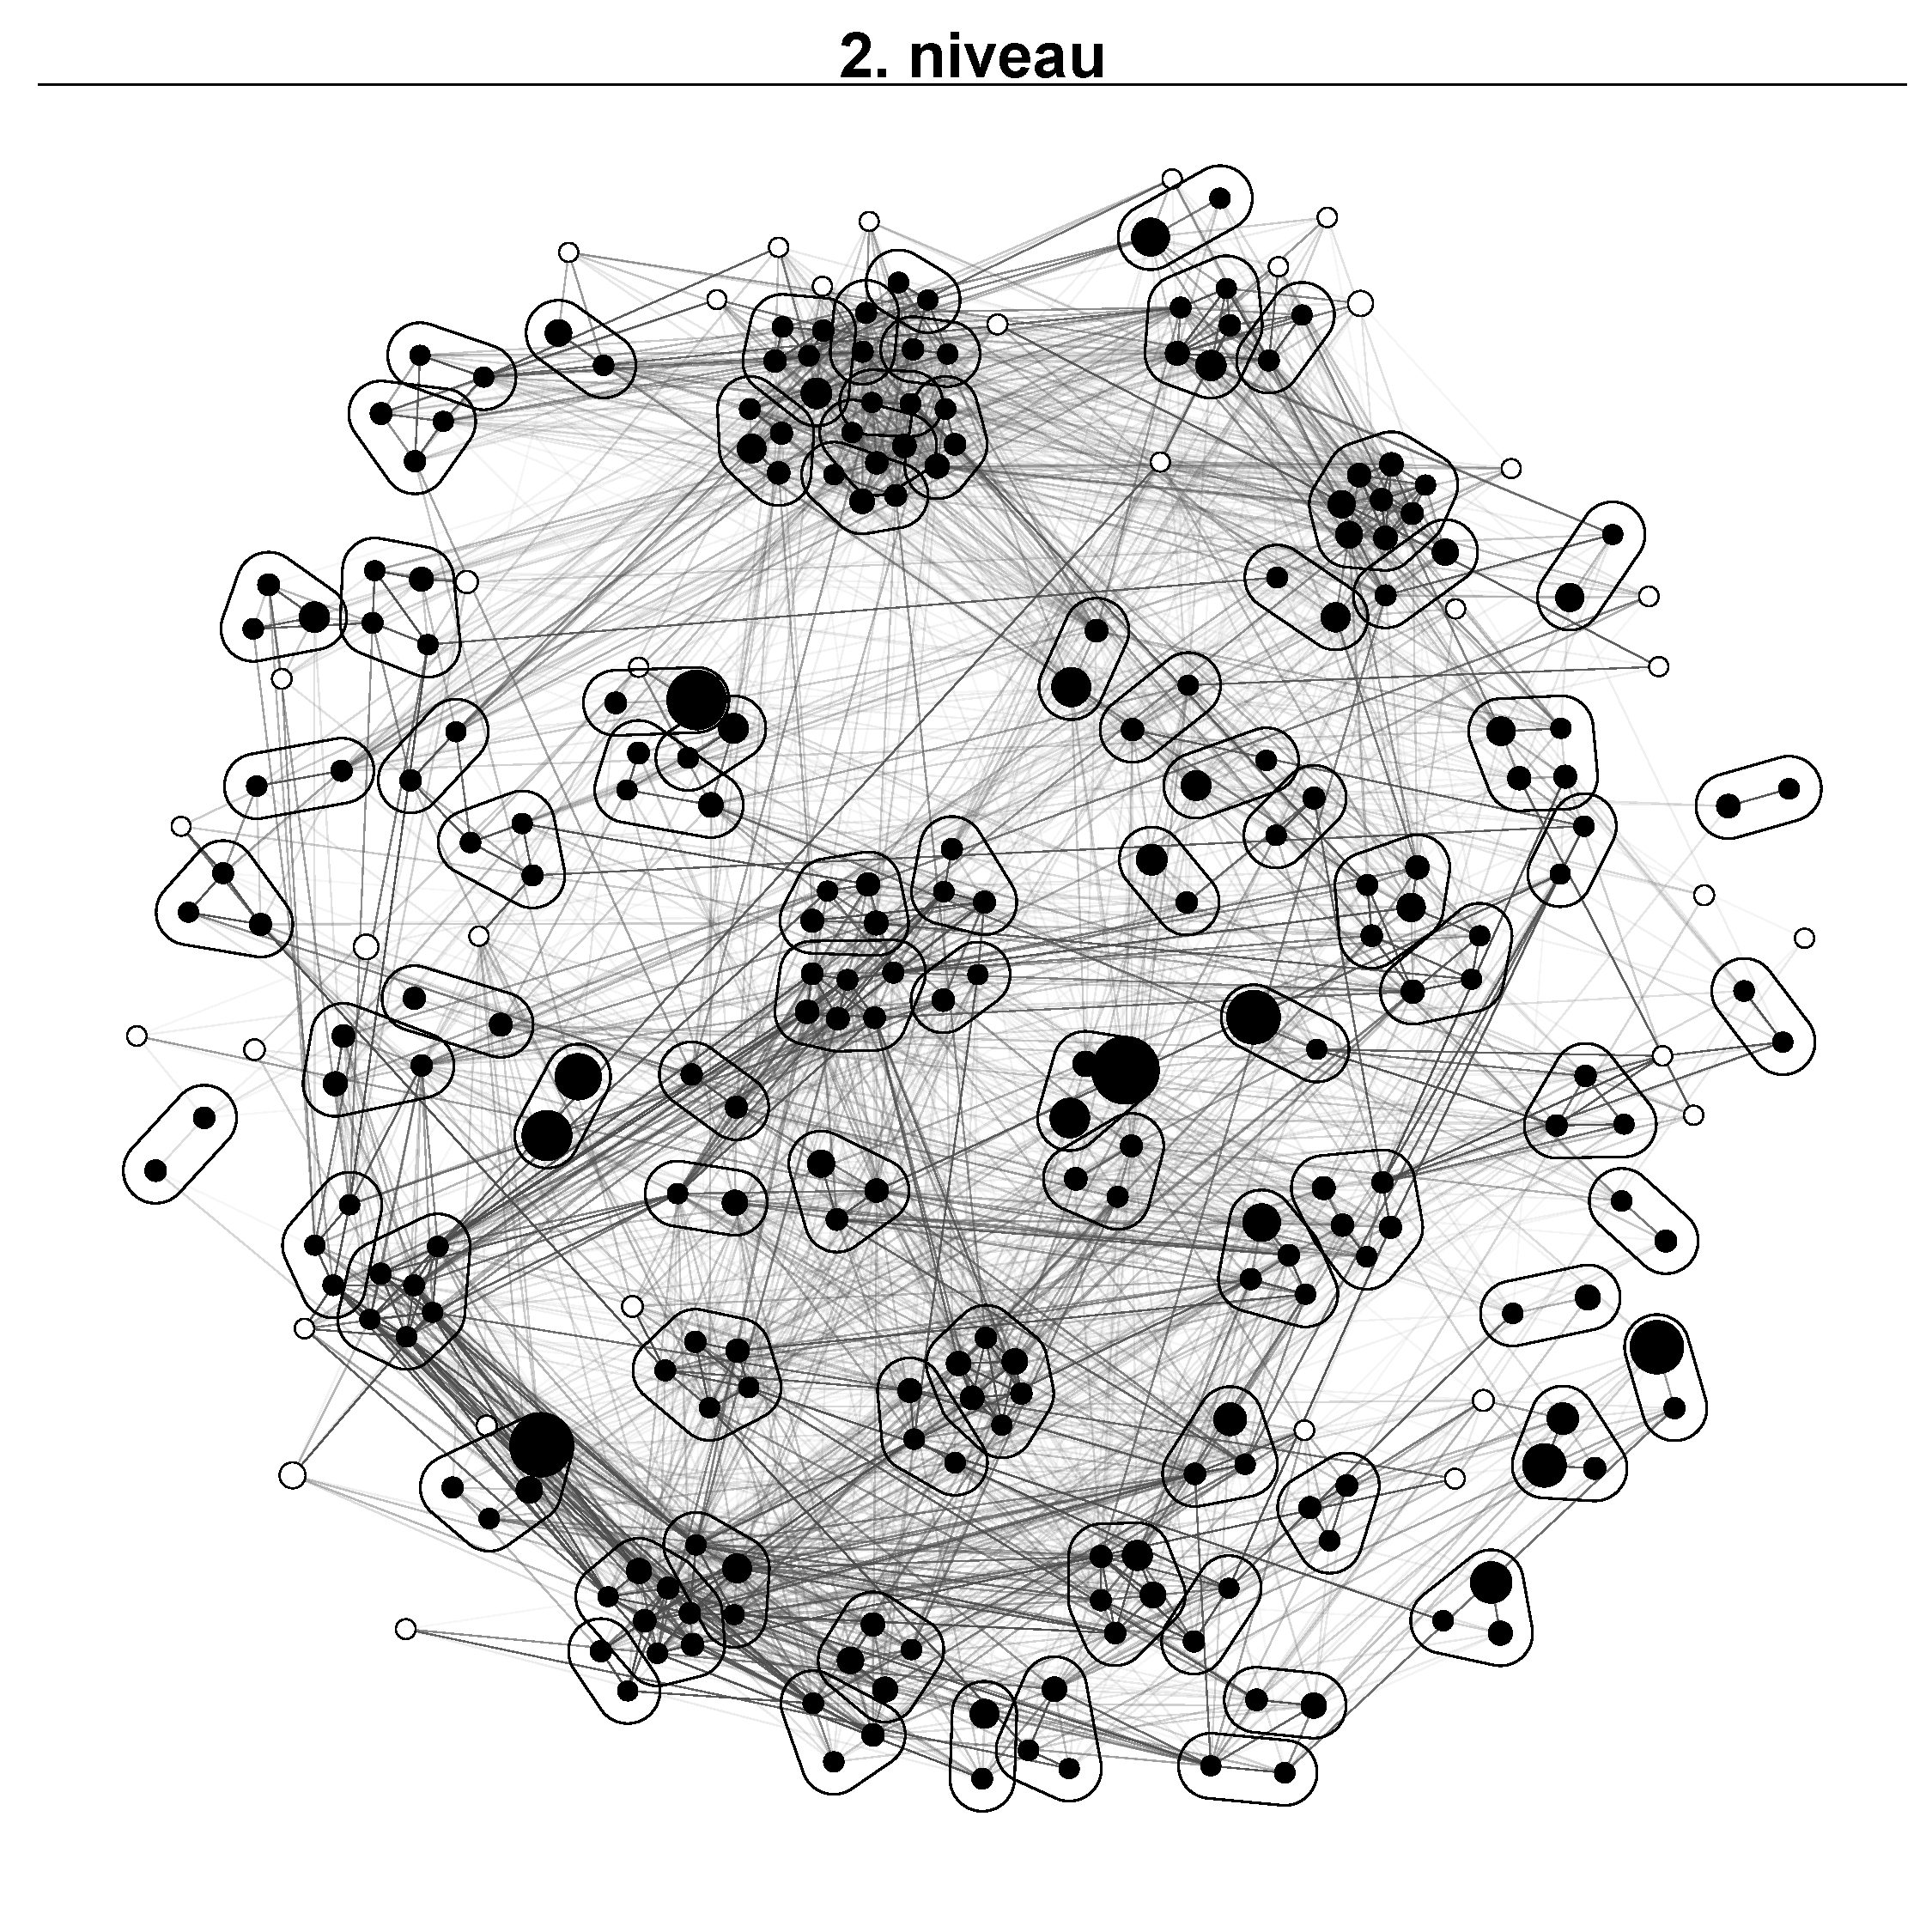
\includegraphics[width=8cm]{fig/netvaerkskort/kort_seg_proces2.pdf}
  \end{center}
  \vspace{-20pt}
\end{wrapfigure}

Den mest markante aggregering i klynger og stigning i intern jobmobilitet fra finder sted i skiftet fra 1. niveau til 2. niveau, og herefter falder effekten af klyngedannelsen på den interne jobmobilitet støt. Af figur \ref{fig_delanalyse1_kort_seg_proces2} fremgår aggreringen. Forskellen på hvide og sorte noder er simpel. Sorte node indikerer at denne node er blevet inkluderet i en ny klynge siden det foregående niveau. Hvid node indikerer at den \emph{ikke} er blevet inkluderet i en ny klynge siden niveauet før. 

På 2. niveau går vi fra de oprindelige 273 fritstående noder til 81 klynger, samt 33 endnu fritstående noder. Det vil sige 114 grupper i alt. Der skelnes i ovenstående tabel ikke mellem enkelte noder og klynger, da klyngernes interne mobilitet jo netop skal erstatte nodernes, og en direkte sammenligning derfor er ønskelig. Antallet af klynger er reduceret med 139 \%, og den gennemsnitlige interne mobilitet i klyngerne er steget med 7 procentpoint.


%%%%%%%%%%%%%%%%%%%%%%%%%%%%%%%%%%%%%%%%%%%%%%
\newpage \subsection{Niveau 3}
%%%%%%%%%%%%%%%%%%%%%%%%%%%%%%%%%%%%%%%%%%%%%%

\begin{wrapfigure}{r}{8cm}
  \vspace{-20pt}
  \begin{center}
   \caption{}
   \label{fig_delanalyse1_kort_seg_proces3}
    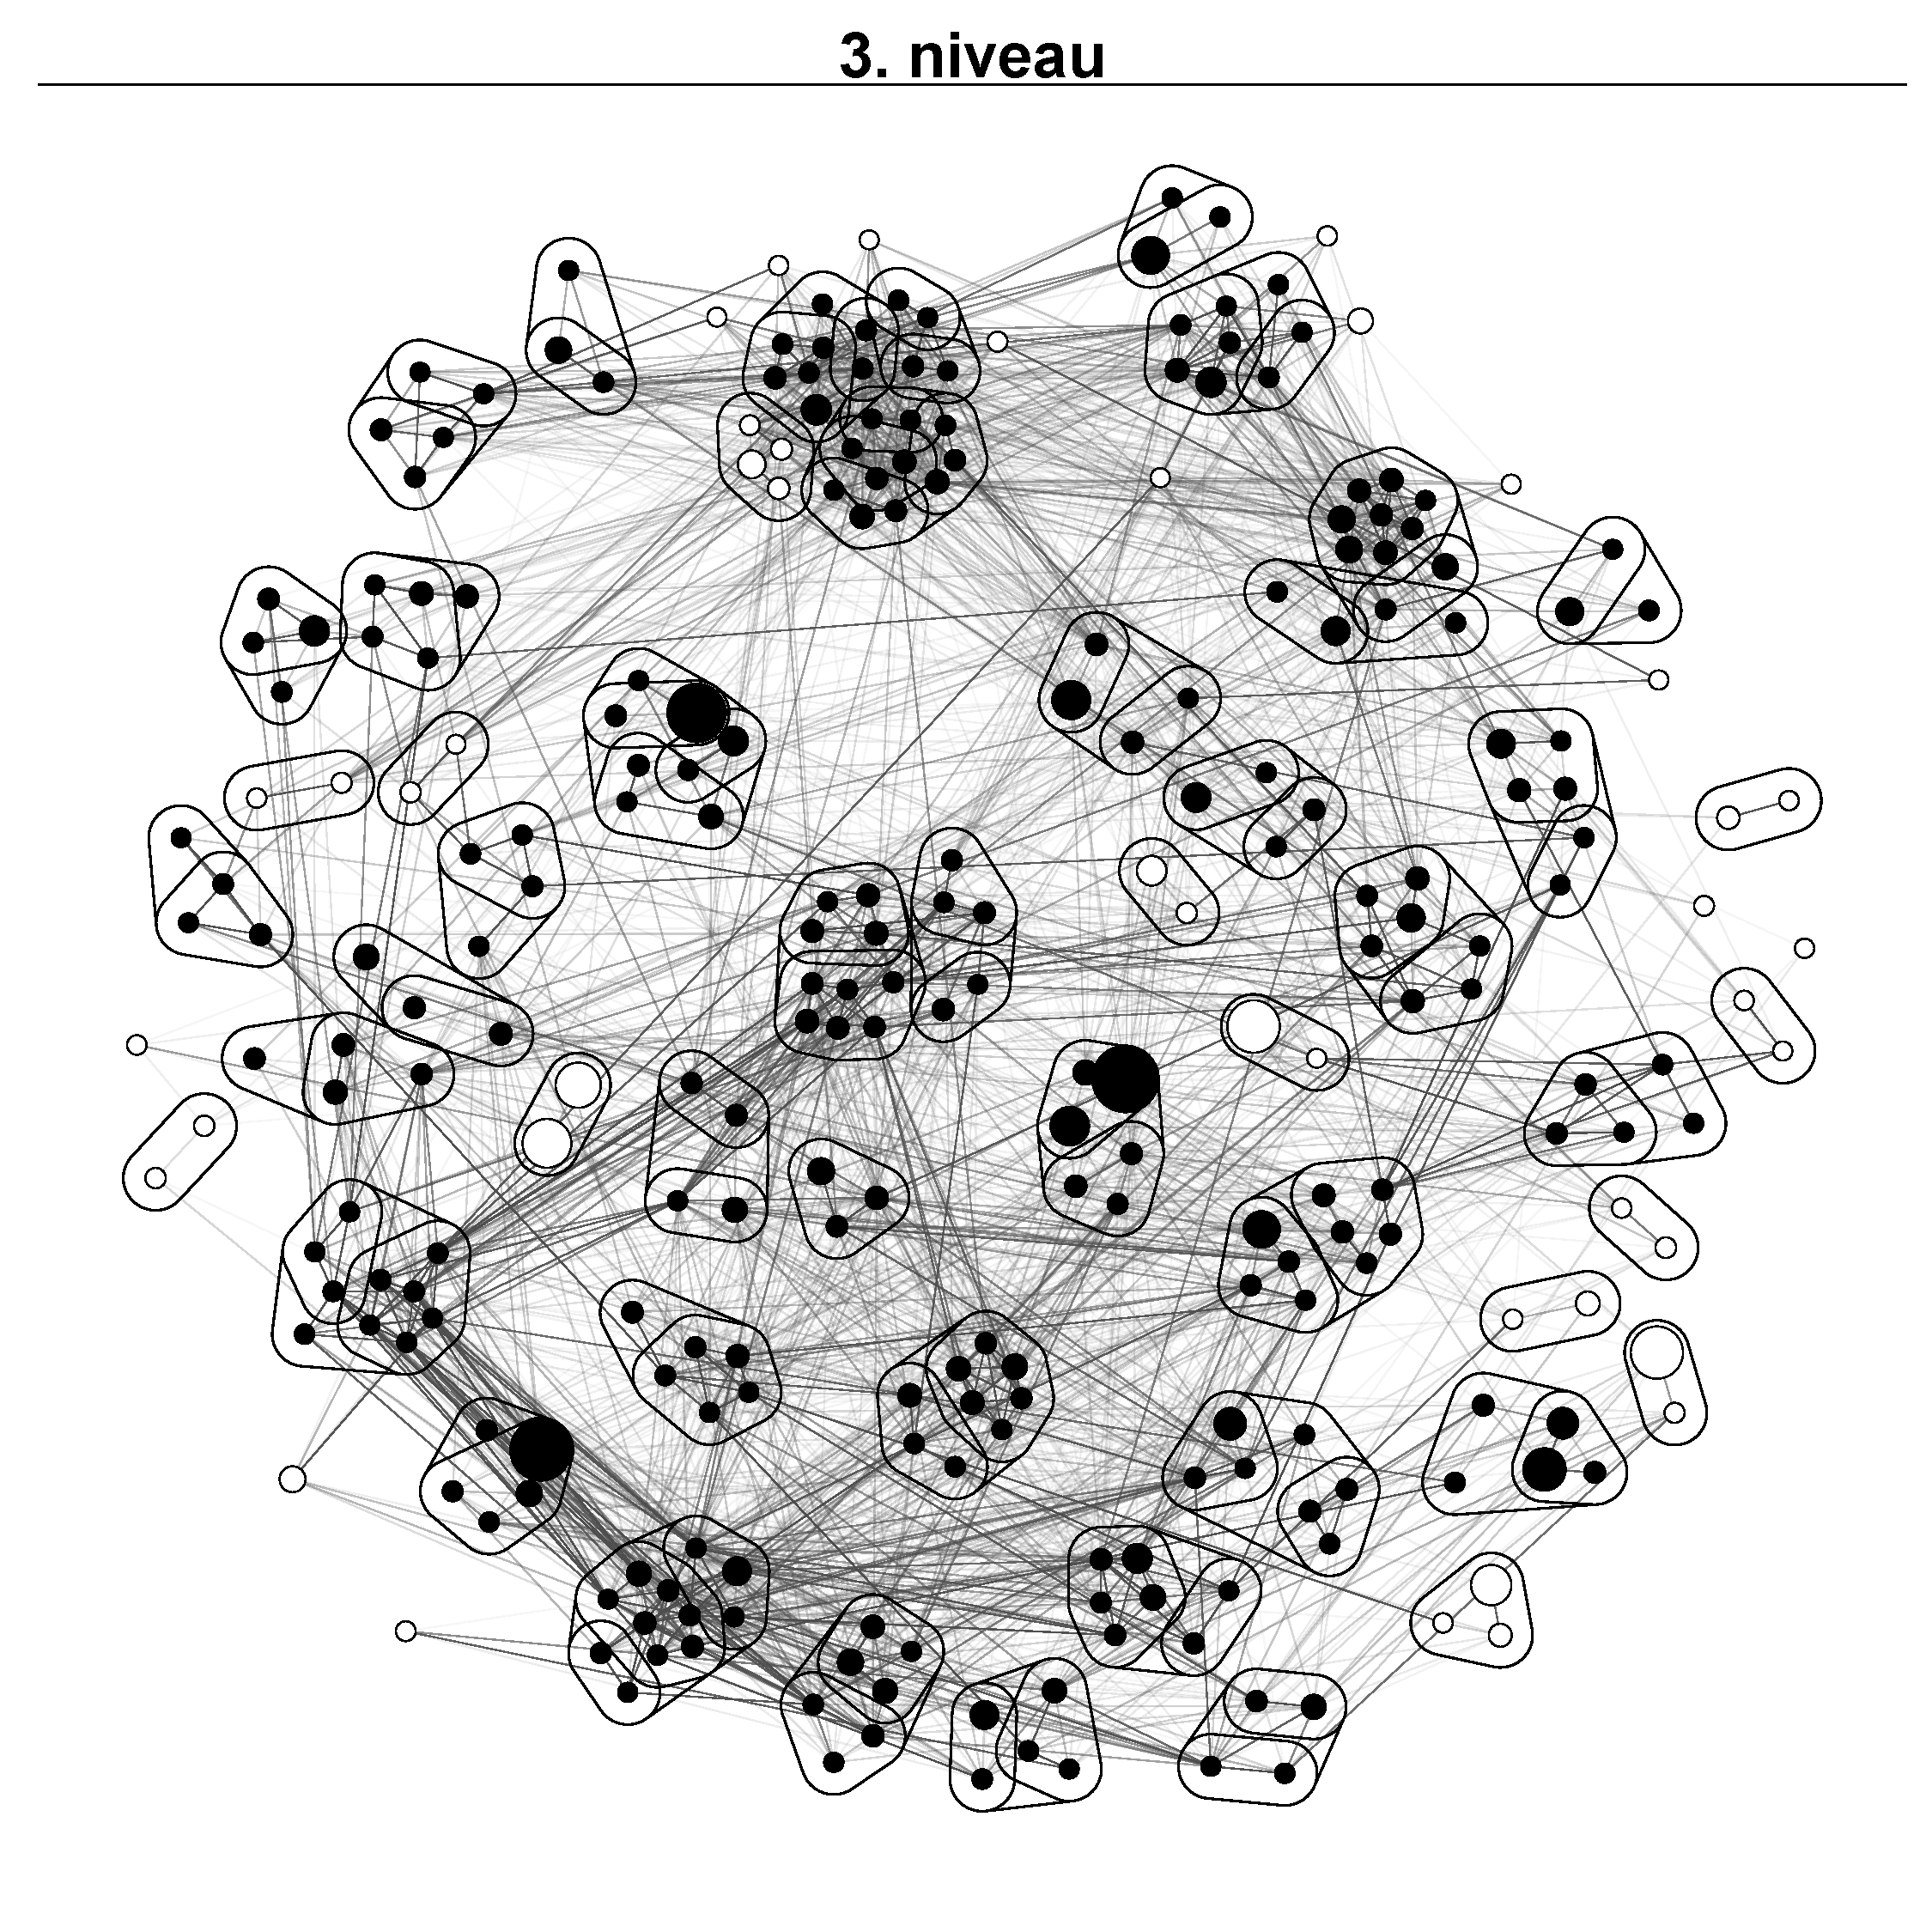
\includegraphics[width=8cm]{fig/netvaerkskort/kort_seg_proces3.pdf}
  \end{center}
  \vspace{-20pt}
\end{wrapfigure}

På 3. niveau, afbilledet i figur \ref{fig_delanalyse1_kort_seg_proces3}, inkluderes 21 enkeltstående noder i klynger, samt en række niveau 2 klynger aggrereres yderligere. Det reducerer antallet af grupper til 68. Stigningen i den gennemsnitlige interne mobilitet kun er på 2 procentpoint. Tilgengæld er reduktionen i antallet af grupper på 68 \%. Det vil sige at kompleksiteten i netværket reduceres, uden at det går udover den interne mobilitet, der er stigende, omend svagt. Det er tendensen fra niveau 3 og frem: Der foretages stadig væsentlige sammenlægninger af klynger og noder til større klynger, men betydning af sammenlægningen på den interne mobilitet er markant faldende. Det ser jeg som udtryk for, at jo længere væk fra den sociale kontekst af det oprindelige job, vi kommer, desto mindre systematik er der i jobskiftet.


%%%%%%%%%%%%%%%%%%%%%%%%%%%%%%%%%%%%%%%%%%%%%%
\newpage \subsection{Niveau 4}
%%%%%%%%%%%%%%%%%%%%%%%%%%%%%%%%%%%%%%%%%%%%%%

\begin{wrapfigure}{r}{8cm}
  \vspace{-20pt}
  \begin{center}
   \caption{}
   \label{fig_delanalyse1_kort_seg_proces4}
    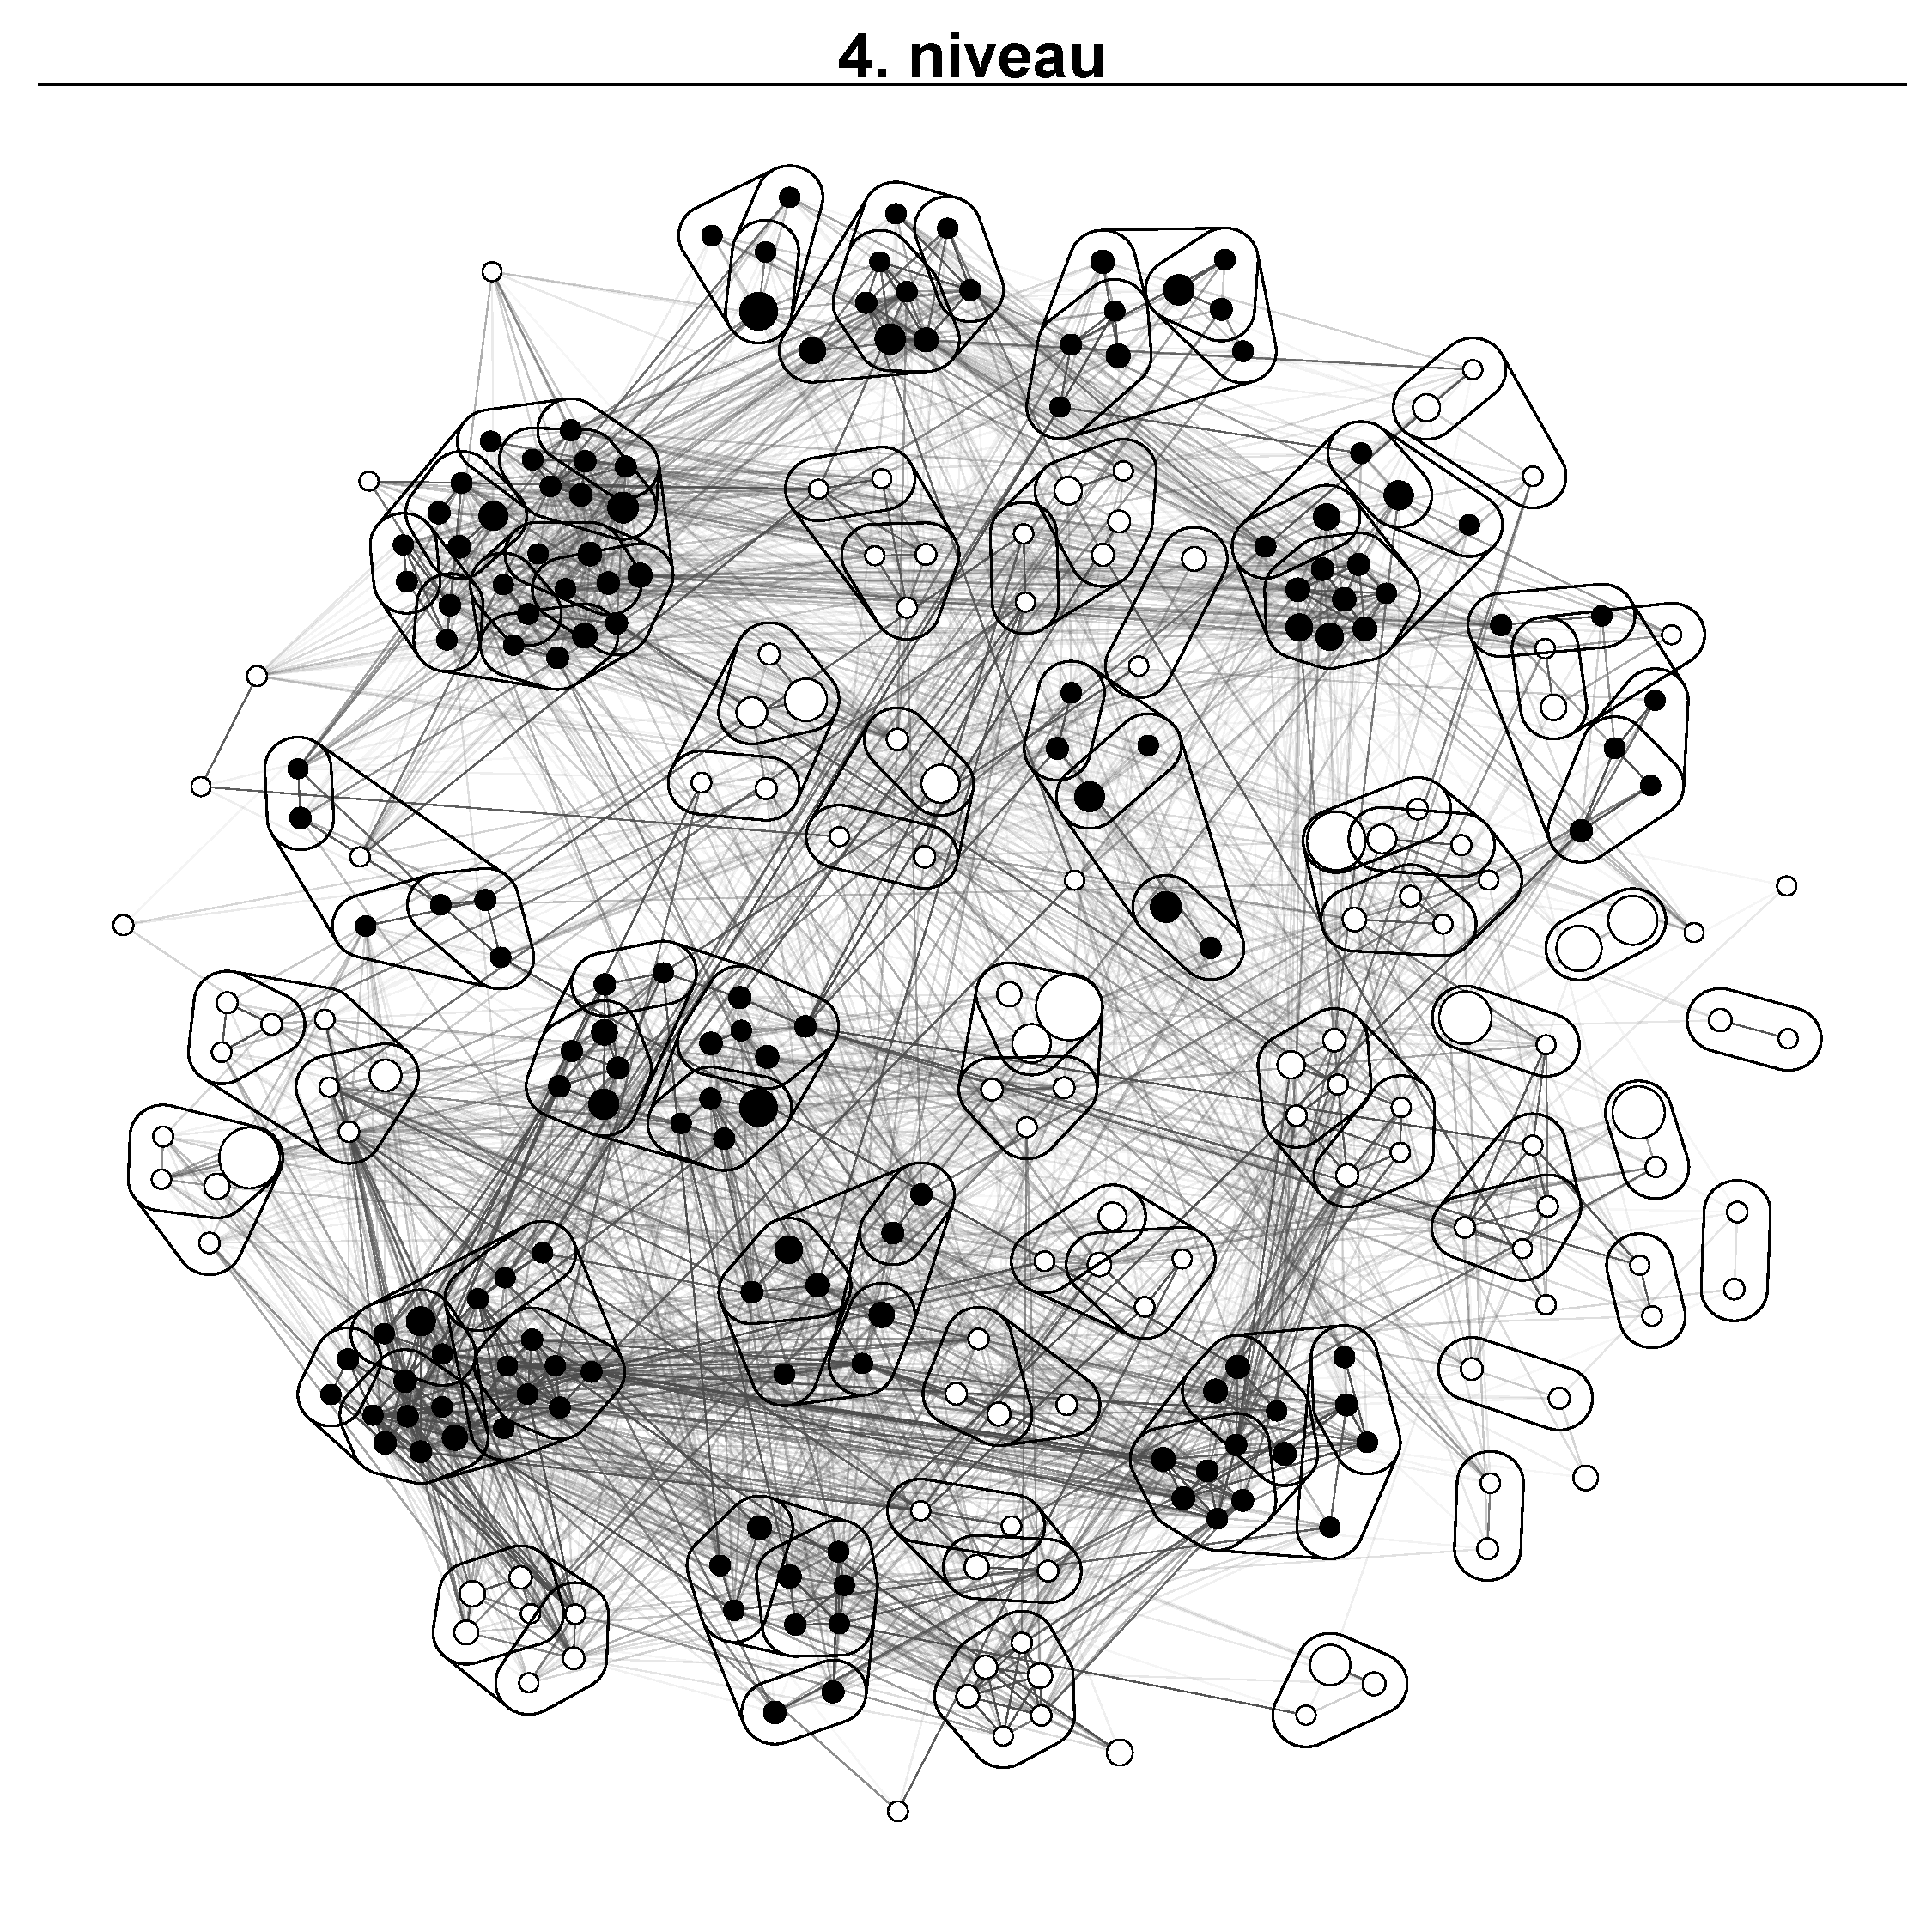
\includegraphics[width=8cm]{fig/netvaerkskort/kort_seg_proces4.pdf}
  \end{center}
  \vspace{-20pt}
\end{wrapfigure}

På 4. niveau skabes 13 nye klynger. Kun en enkelt af disse sker i en sammenlægning med en enkeltstående node. Resten er tidligere klyngedannelser. 
Der er nu 53 grupper hvoraf 13 er enkelte beskæftigelser. Den interne mobilitet er steget med et enkelt beskedent procentpoint.
%
\footnote{Selvom en 1 procent stigning kan virke af lidt viser effektforskninger, fx Andrade, at er bare den 1 1/2 procent han kan finde i indkomstforskelle meget. De forklarer ofte kun 5-10 procent af den totale variation.}” \parencite[302]{Weber1978}. }%
%
Antallet af grupper er tilgengæld reduceret med 28 \%, lidt over $\nicefrac{1}{4}$. Det er på dette niveau, at sammenlægningerne binder allerede store klynger sammen, og vi får udvidede klynger med en betragtelig mængde forskellige arbejdsfunktioner samlet under ét.

Disse klynger af arbejdsfunktioner er ikke baseret på den \emph{teknisistiske vision}, som Grusky advarer imod, og heller ikke en a priori teoretisk opdeling. Inddelingen er istedet baseret på den sociale nærhed, der antages at findes mellem jobs, hvor mobilitet er “let og typisk” , som Weber siger det i sin definition af hvad der udgør en social klasse. %kalder det, sin beskrivelse af (et af) de definerende træk ved social klasse: Individuel mobilitet% Det her skal nok stå i teori-afsnittet, og så henvises til her i stedet. \#todo
%
\footnote{Der er naturligvis flere elementer end individuel jobmobilitet på spil. Det fulde citat lyder: “\textit{A »social class« makes up the totality of those class situations within which individual and generational mobility is easy and typical.}” \parencite[302]{Weber1978}. }%
%
En enkelt klynge, Moneca ville have lavet på dette niveau, har jeg valgt at underkende. Det skyldes at den ville have fået en stilængde på 4. I SNA er stilængde den korteste vej, der er mellem to noder. Dette er meget væsentligt for vurderingen af dannelsen af klynger. Med en stilængde på 4 bliver klynget for opdelt... Derfor vurderes kvaliteten af denne klynge dårlig. Der er i alt blivet splittet fire klynger op. 


%%%%%%%%%%%%%%%%%%%%%%%%%%%%%%%%%%%%%%%%%%%%%%
\newpage \subsection{Niveau 5 \label{delanalyse1_endelige mobilitetskort}}
%%%%%%%%%%%%%%%%%%%%%%%%%%%%%%%%%%%%%%%%%%%%%%

Det 5. niveaeu er det sidste niveau, da Moneca-algoritmen ikke kan aggregere klynger på et højere niveau end det. Vi mindes fra gennemgangen af Moneca-proceduren på side  \pageref{metode_monecastepbystep}, at det betyder, at Moneca ikke kan finde nogle noder eller tidligere klynger, hvor der er intern mobilitet mellem  \emph{alle} klynger fra niveauet tidligere. %check lige op på det med Anton \#todo 
I skiftet fra niveau 4 sker der tre aggregeringer: En inklusion af en enkelt node i en niveau 4- klynge, samt en større sammenlægning af en niveau 4- og en niveau 3-klynge. Det bringer os ned på 12 enkeltstående noder, samt 39 klynger. 

\begin{figure}[H]
\begin{centering}
  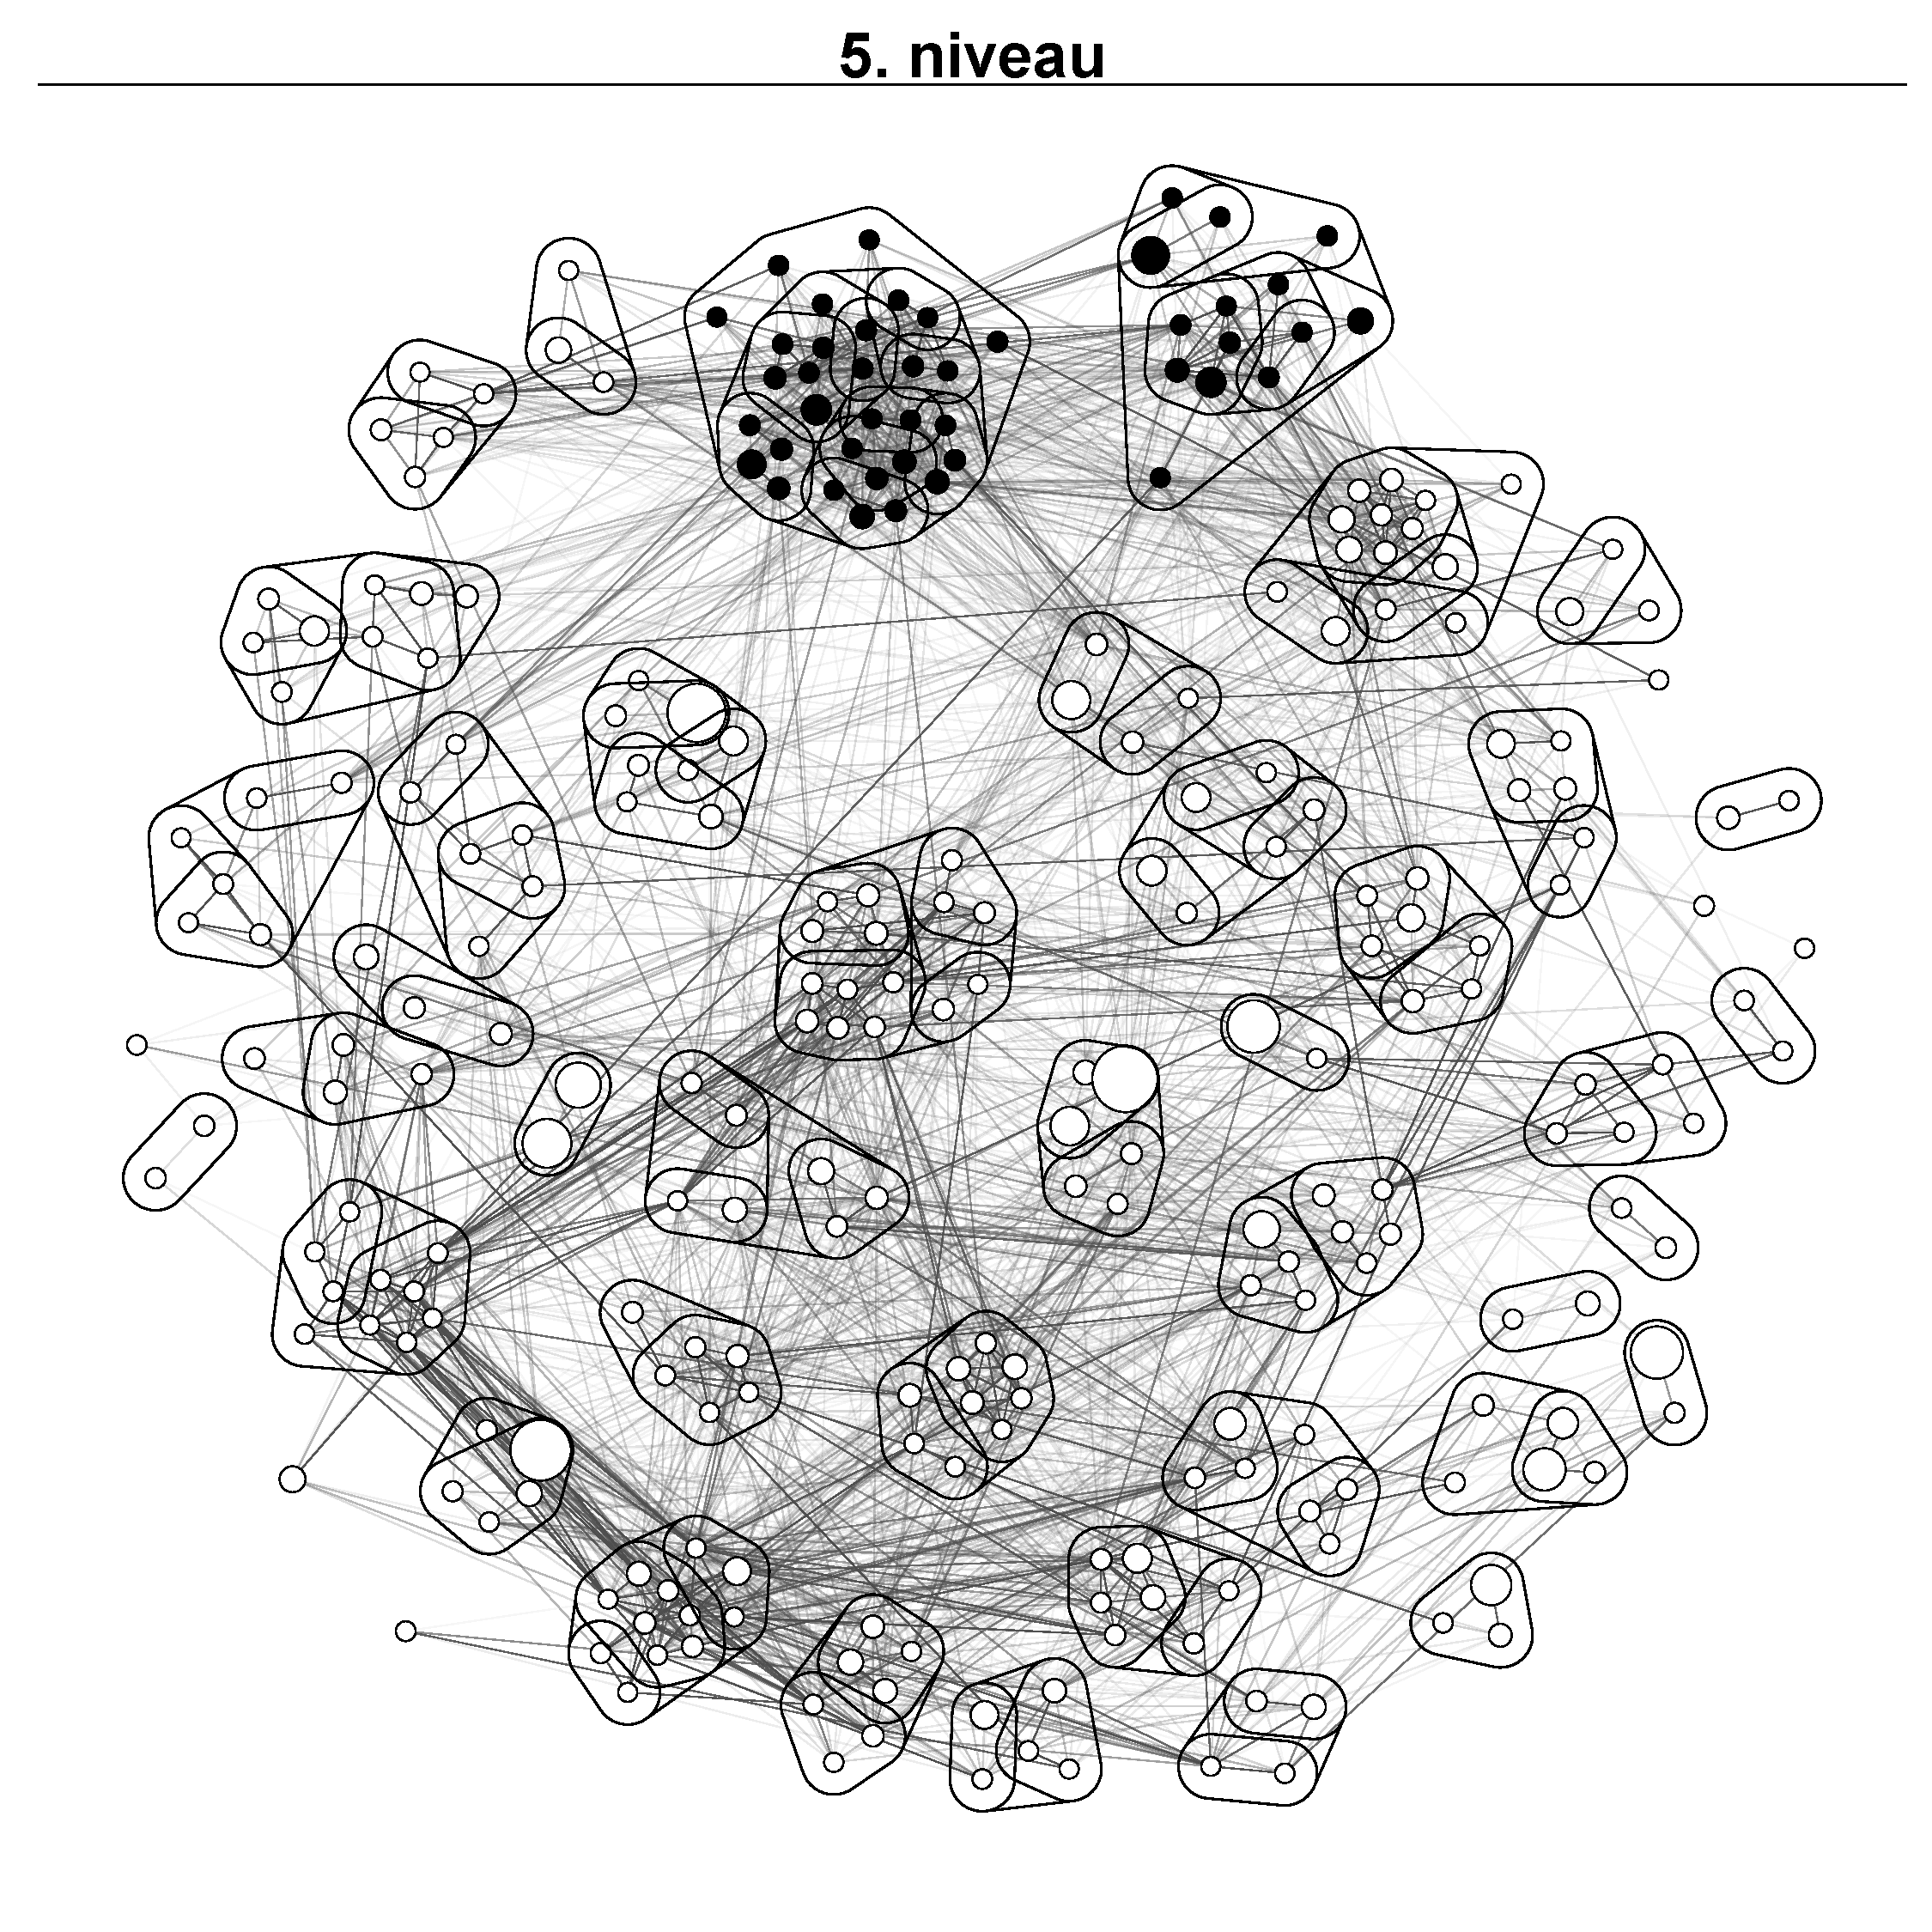
\includegraphics[width=10 cm]{fig/netvaerkskort/kort_seg_proces5.pdf}
  \label{fig_delanalyse1_kort_seg_proces5}
  \caption{}
\end{centering}
\end{figure}

Her er forbedringen i den interne mobilitet endnu en gang på et enkelt procentpoint. En gennemsnitlig intern mobilitet på 79 \% er hvad det er hvad det er muligt at komme frem til. Dette forekommer rimeligt og acceptabelt, og en stigning på 11 procentpoint i den interne mobilitet fra niveau 1 til niveau 5 vurderer jeg som ganske tilfredsstillende, når det endelige resultat forklarer omtrent $\nicefrac{4}{5}$ af mobiliteten. Dette er i god overenstemmigelse med tidligere undersøgelser, der viser at hovedparten af skift i job sker indenfor relativt afgrænsede klynger \parencite[124]{BojeToft1989}. 

Den oprindelige 273 x 273 mobilitetstabel nu er reduceret til en mere overkommelig 51 x 51 mobilitetstabel. Ud af disse 51 kategorier er 12 enkelstående noter, der ikke er sammenlagt med andre noter, mens 39 er klynger. Tabel \ref{tab_delanalyse1_noegletalniveau1og5} viser yderligere centrale mål. Disse viser tydeligt at aggregeringen har skabt færre kategorier med højere intern mobilitet.

%!TEX encoding = UTF-8 Unicode
%!TEX root = ../report.tex
% Table generated by Excel2LaTeX from sheet 'delanalyse1_noegletalniveau1og5'
\begin{table}[htbp]
  \centering
  \caption[Nøgletal for første og sidste niveau i klyngedannelsen]{Nøgletal for (det uaggregerede) niveau 1 og (det endelige) niveau 5}
  \resizebox{.8\textwidth}{!}{%
    \begin{tabular}{lcccccc}
          &       & gns. intern & sd afvigelse  &       &       &  \\
    Niveau & grupper &  mobilitet & 
\emph{\tiny{(i procentpoint)}} & median & min   & max \\
    \midrule
    1. niveau & 273   & 68\%  & 12    & 68\%  & 43\%  & 97\% \\
    5. niveau & 47    & 81\%  & 10    & 80\%  & 54\%  & 96\% \\
    \bottomrule
    \end{tabular}}%
  \label{tab_delanalyse1_noegletalniveau1og5}%
\end{table}%


Medianen på det 1. niveau er på 79 \%, mens det på 5. niveau er steget til 80 \%. Standardafvigelsen for den interne mobilitet på det 1. niveau er på 12 \%, mens den på det 5. niveau er på 10 \%. At standardafvigelsen er faldet og medianen er steget, er vigtigt, fordi det fortæller os at gennemsnittet ikke er trukket op via enkelte klynger.  Det er en generel forbedring af mobilitetsstrukturen. Det ses også ud fra minimumværdierne. Hvor de laveste værdier tidligere lå på lidt over 40 \%, ligger de nu på lidt over 50 \%. På de 3 centrale mål for kontinuerte variable (Find henvisning Malchow-Muller \#todo) er der sket en forbedring. 5. niveau forklarer \emph{mere} mobilitet, og kategoriernes interne mobilitet svinger \emph{mindre} om gennemsnitsmobiliteten end i kategorierne på 1. niveau. Det er meget tilfredsstillende, da det indikerer at et højere aggregeringsniveau ud fra Monecas beslutningsprocedure forklarer \emph{hvor} mobiliteten løber hen, når den bevæger sig udenfor de oprindelige kategorier.  % Det er jo sådan set også det, den er designet til, kunne man indvende. Men det tilfredsstillende her er at helt op til \emph{det 5. aggregreringsniveau} er der stadig en bedre forklaringskraft end på de tidligere niveauer. Man kunne forestille sig at for mange kompromisser med sammenlægninger - genkald argumentet fra side ??(det om at der lægger noder sammen der rent faktisk ikke hænger sammen \#todo) ville fungere kontraproduktivt over et vist niveau, men det er altså ikke tilfældet. % ved ikke helt om det her argument egentligt holder -vil en større sammenlægning ikke bare automatisk give bedre forklaring? Nej! for hvis en node nu har meget mere udveksling med en node udenfor det, den er lagt sammen med, så ville det jo godt kunne trække ned. Men det sker ikke her, altså er det en god sammenlægning. Tror jeg. 

Fra 3. niveau og frem er klyngedannelsens primære funktion at danne større klynger, det vil sige reducere kompleksiteten i jobstrukturen. Visse kategorier indeholer langt flere beskæftigede end andre, og kan derfor anses som mere væsentlige sammenlægninger. Vi får dermed nogle klynger, der antalsmæssigt beskæftiger store dele af den danske befolkning. Dette vil jeg mene er et andet vigtigt parameter i klyngedannelsen. Det vil ikke blive gennemgået nøje her, og vil istedet blive præsenteret i Delanalyse 2 på side \pageref{kap_delanalyse2_socialeprocesser}.

I dette afsnit er aggreringen fra niveau til niveau blevet beskrevet med henblik på at vrdere kvaliteten af delmarkederne. Det er stadigvæk klart, at der ikke er tale om dual eller tredeling af arbejdsmarkedet \parencite{Piore1980, Gordon1982}, men men tydeligvis tale om en meget mere faktioneret arbejdsmarkedet som Boje og igen Toubøl taler om \parencite{Boje1985, Touboel2013}. I det følgende sættes der fokus på den interne mobilitet, fordi det er et helt centralt begreb som forklaring af opdelingen af delmarkederne.


%%%%%%%%%%%%%%%%%%%%%%%%%%%%%%%%%%%%%%%%%%%%%%
\section{Den interne mobilitet i klyngerne \label{analyse_deskriptivt_within_mob_seg}}
%%%%%%%%%%%%%%%%%%%%%%%%%%%%%%%%%%%%%%%%%%%%%%

Jobmobilitet fremgår som mobilitet internt i de 51 klynger og eksternt mellem klynger. 79 \% af al mobilitet foregår inden for klyngerne. At der blot er 21 \% af al mobilitet mellem klyngerne viser altså tydeligvis barrierer for mobilitet mellem klyngerne.  % Den interne og eksterne mobilitet er drøftet teoretisk i afsnit ?? og den metodiske implementering er drøftet i afsnit ?? \#todo.

For Boje er det helt centralt, at der er begrænset mobilitet mellem de enkelte klynger. Og for Weber er det vigtigt, at der er, at den sociale nærhed, der antages at findes mellem jobs, hvor mobilitet er “let og typisk”.

Den interne mobilitet for hvert klyng er præsenteret i et netværkskort på figur \ref{fig_analyse_deskriptivt_kort_intern_mob_seg}, \pref{fig_analyse_deskriptivt_kort_intern_mob_seg}).

\underline{Størrelsen på en node} repræsenterer ganske simpelt hvor mange personer, der i gennemsnit er i beskæftiget indenfor jobkategorien i årrækken 1996-2009%
%
\footnote{Når jeg fra nu af taler om hvor mange der er beskæftigede, er det underforstået at der er tale om det gennemsnitlige antal \emph{indenfor årrækken 1996-2009}, med mindre det eksplicit fremhæves at der er tale om noget andet.}%
%
Den største kategori, \texttt{5220: Ekspedient-, kasse- og demonstrationsarbejde} indeholder 114.869 personer i gennemsnit, svarende til 4,9 \% af det totale antal beskæftigede. Mens den mindste, \texttt{7346: Serigrafisk arbejde} indeholder 504 personer, svarende til 0,02 \% af det totalen 
%
\footnote{Der er ikke tale om et korrekt repræsenteret størrelsesforhold mellem de forskellige jobkategorier. Det er for komplekst til visuel afkodning i et allerede informationstungt netværkskort, da de mindste noder ville blive meget små og de store noder meget store. Derfor har jeg valgt et størrelsesforhold mellem noderne, der ikke er 1:1 med deres reelle forskelle i størrelse, og som alligevel giver en fornuftig fornemmelse for disse størrelsesforhold. Man skal dermed se både farve af forbindelserne og nodernes størrelse som en grov målestok af den variabel, den repræsenterer. Med vægten lagt på nem visuel afkodning, fremfor korrekt gengivelse af datakompleksisteten.}%

\newgeometry{left=-0.01cm,bottom=0.1cm}
\begin{figure}[H]
\begin{center}
	\caption{Intern mobilitet for klyngerne.}
	\label{fig_analyse_deskriptivt_kort_intern_mob_seg}
	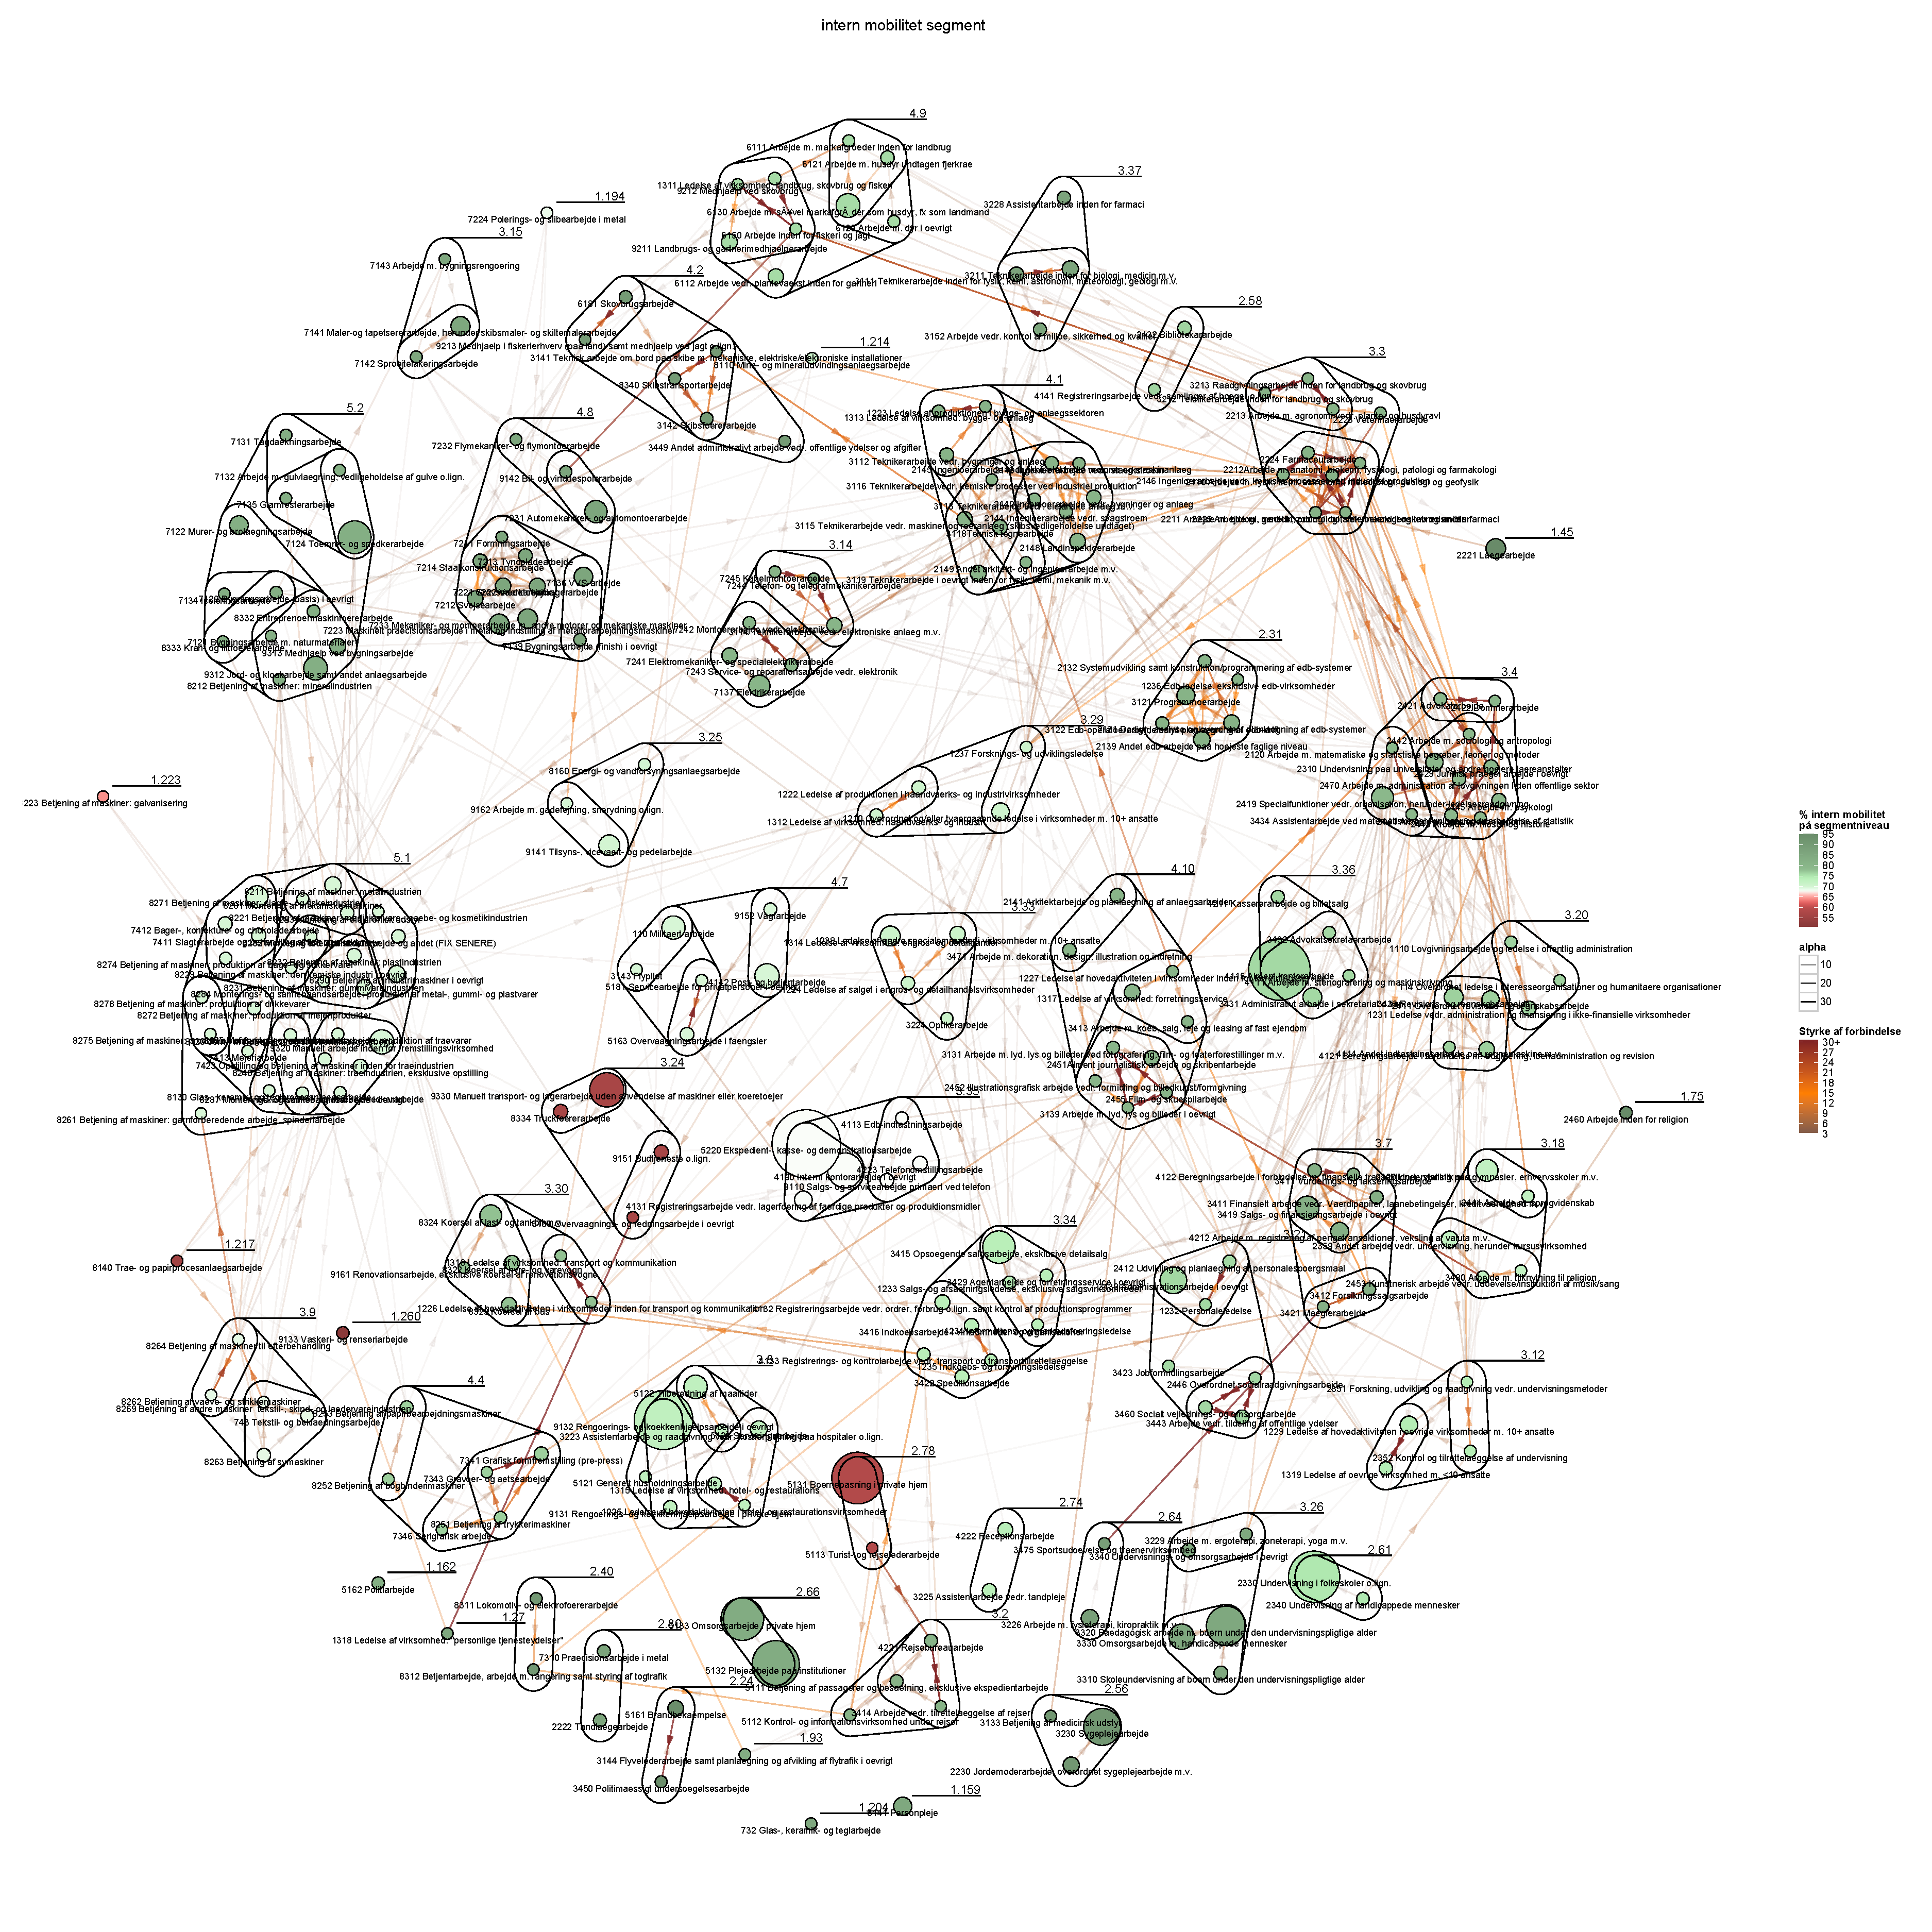
\includegraphics[width=1.0\textwidth]{fig/netvaerkskort/kort_intern_mob_seg.pdf}
	\centerline{ \tiny{Kilde: Nielsen-Gravholt og Begtrup-Bright}}
\end{center}
\end{figure}
\restoregeometry

Styrken af mobilitet er først og fremmest ved \underline{nodernes farve}. Farven går fra mørkerød, til hvid, til mørkegrøn betyder det, hvor stor eller lille den intene mobilitet er. De mørkerøde klynger markerer en intern mobilitet på mellem 50 og 60 \%, mens den derfra og op til 67 \% antager en stadigt svagere lys rød, indtil den er ren hvid ved 68 \%. De grønner klynger markerer en intern mobilitet på mellem 68 \% og 76 \%, som bliver den stadig mere grøn, for ved 80 \% at være helt mørkegrøn.
%
\footnote{Da der er tale om en gradient, er skiftet i farve en kontinuer overgang. Skiftet i farve er motiveret af min egen vurdering, baseret på de deskriptive værdier for den interne mobilitet gennemgået i det foregående afsnit. Der findes ingen tidligere brug af Moneca algoritmen, hvori dette indgående bliver analyseret. Jeg har besluttet mig for, at en mobilitet mellem erhvervene i en klynge på 68 \% og derover, er en fornuftig tærskel. Det skyldes at nodernes interne mobilitet på det (uaggregerede) niveau 1 er på 68 \%, og jeg derfor anser det som et fornuftigt kriterie. Det ses at langt de fleste klynger overholder denne beslutningsregel. 3 klynger og 3 noder ligger under 68 \%. Det betyder ikke at disse klynger nødvendigvis skal forkastes. Vi ser nærmere på disse klynger og vil vurdere deres kvalitet løbende. Der er altså ikke er tale om en statistisk test med et vist signifikansniveau, men min egen tentative vurdering. Og selv med de vedtagne signifikansniveauer i statistiske test, eksempelvis p-værdier i en T-test eller en F-test,  der advarer litteraturen om ikke at tolke disse tærskelværdier som skrevet i sten, men som nyttige konventioner (find henvisning, Gujarati og Malchow-Møller \#todo) (blah blah).}%
%
\underline{forbindelsens farve} markerer som beskrevet i afsnit \ref{metode_relativrisiko} forbindelsernes styrke målt ved den relative risiko. Et forholdsmål, der udtrykker mobiliteten fra en kategori til en anden, givet den relative størrelse af antallet af beskæftigede i kategorien. Det er styrken af denne relative risiko (RR), der afgør farven på forbindelserne, der kan antage tre nuancer: Helt lysegrå angiver en RR på 3%
%
\footnote{Husk på fortolkningen af relativ risiko:  det vil sige, at der er ved en lysegrå forbindelse er 3 gange så stor sandsynlighed for mobilitet fra den forladte beskæftigelse til den nye beskæftigelse, i forhold til hvis der var tale om et arbejdsmarked med helt fri bevægelse.}%
%
. Helt orange angiver en RR på 15. Helt mørkerød angiver en RR på 30 \emph{ eller derover}. I bestemmelsen af klyngerne, er alle forbindelser med en RR på over 1 medtaget som en forbindelse. På det visuelle kort er den informationsmængde upraktisk. Det bliver umuligt at aflæse den underliggende systematik i hvilke forbindelser, der værd at lægge mærke til. Enkelte forbindelser har RR-værdier på flere tusinde, men de fleste langt lavere: Medianen er på 2,1. En relativ risiko på 3 svarer cirka til den 65. percentil, og 15 er cirka den 90 percentil. 30 svarer til cirka den 92,5'te percentil, og er ikke valgt ud fra denne, men bestemt ud fra det punkt, hvor der sker en stigning i styrken af forbindelserne. 

Forbindelserne er desuden retningsbestemte, hvor pilene på kortet angiver retningen af mobiliteten mellem noderne.
%
\footnote{Ovenstående er bortset fra nodernes farver de generelle retningslinjer for netværkskortene.}%
%
\begin{wrapfigure}{r}{6cm}
  \vspace{-20pt}
  \begin{center}
    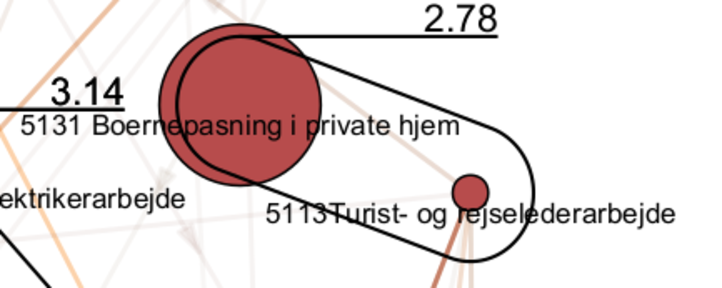
\includegraphics[width=6cm]{fig/segzoom/seg_2_78.pdf}
   \caption{}
   \label{fig_delanalyse1_zoom_2_78}
  \end{center}
  \vspace{-20pt}
\end{wrapfigure}
%

%%%%%%%%%%%%%%%%%%%%%%%%%%%%%%%%%%%%%%%%%%%%%%
\subsection{Klynge \emak{s2.78}: Børnepasning i private hjem, samt turist- og rejseledere}
%%%%%%%%%%%%%%%%%%%%%%%%%%%%%%%%%%%%%%%%%%%%%%

. Hvis vi kigger på klynge \emak{s2.78}, kan vi se at den består af børnepasning i private hjem, samt turist- og rejseledere. Jobkategorierne har en intern mobilitet på henholdsvis  59 \% og 47 \%, altså ganske lavt sammenlignet med den gennemsnitlige interne mobilitet for alle jobkategorierne, der er på 68 \%.  Begge jobs er indenfor hovedgruppe 5 i DISCO-nomenklaturet: \texttt{salgs-, service- og omsorgsarbejde}. Det er klassificeret som tilhørende færdighedsniveau 2. Det er arbejde, der ifølge Danmarks Statistik er klassificeret som ISCEDs færdighedsniveau 2, hvilket betyder at det kræver uddannelse “på grundniveau” \parencite[tabel 1]{DSTDISCO88}. Det er en klar indikator på at de formelle sociale lukningsmekanismer i disse erhverv er stærkt begrænsede.

En oplagt årsag er at beskæftigelserne i denne type klynger simpelthen er jobs, der af den ene eller anden årsag har en karakter, der gør at folk sjældent opholder sig længe i dem. Det kunne man kalde en socialt betinget lav intern mobilitet. Det kunde, eller ansættelserne så usikre, at man ikke bliver i dem længe af gangen. Hvis arbejdet har denne karakter, må man forvente, at de sociale lukningsmekanismer næppe er særlig højtudviklede. Den mest legitime af disse, i moderne samfund, må være adgangsgivende uddannelse. Vi vil derfor forvente at finde enten ufaglært fag, eller fag med lave uddannelsesmæssige krav. Det kan altså have en social årsag at den interne mobilitet er lav. Det er vigtigt at få afklaret, da disse klynger kan risikere ikke at kunne betegnes som klynger i teoretisk forstand, hvis mobiliteten mellem dem ikke er hyppig.  

Det er imidlertidigt ikke tilstrækkeligt til at forstå hvorfor denne klynge ikke fungerer som delmane være ufaglærte jobs som her, der typisk henvender sig til unge og studerende. Eller ufaglært, sæsonbetinget arbejde, samt jobs der simpelthen er så  rked. Der er andre klynger på kortet, hvor uddannelseskravene er lave, men hvor den interne mobilitet er høj. Et nærliggende eksempel er De mørkerøde klynger markerer en intern mobilitet på mellem 50 og 60 \%, mens den derfra og op til 67 \% antager en stadigt svagere lys rød, indtil den er ren hvid ved 68 \%. De grønner klynger markerer en intern mobilitet på mellem 68 \% og 76 \%, som bliver den stadig mere grøn, for ved 80 \% at være helt mørkegrøn.klynge \emak{s2.66}, som er grøn. 


%%%%%%%%%%%%%%%%%%%%%%%%%%%%%%%%%%%%%%%%%%%%%%
\subsection{Klynge \emak{s2.66}: Omsorgsarbejde i private hjem og plejearbejde på institutioner}
%%%%%%%%%%%%%%%%%%%%%%%%%%%%%%%%%%%%%%%%%%%%%%

Jobs i klynge \emak{s2.66} befinder sig ligeledes i hovedgruppe 5, men den interne mobilitet, både i klyngen og blandt jobbene selv, er meget høj. Børnepasning i private hjem ligger ganske tæt på arbejdsfunktionerne i klynge \emak{s2.66}. Så tæt at de på et 3-cifret Disco niveau er kategoriseret ens, det er kun på det 4. ciffer at de adskiller sig fra hinanden. klynge \emak{s2.66} har en intern mobilitet på 83 \%, væsentligt højere end klynge \emak{s2.78}. Det kan ikke forklares ud fra formelle krav. 

%
\begin{wrapfigure}{r}{6cm}
  \vspace{-20pt}
  \begin{center}
    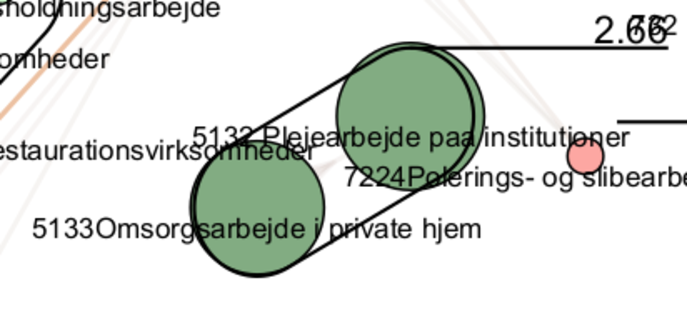
\includegraphics[width=6cm]{fig/segzoom/seg_2_66.pdf}
   \caption{}
   \label{fig_delanalyse1_zoom_2_66}
  \end{center}
  \vspace{-20pt}
\end{wrapfigure}
%

Børnepasning i private hjem har tilsyneladende en noget anden social profil. Den interne mobilitet er meget lavere, og den ligger sammen med turist- og rejseleder, der også befinder sig i hovedgruppe 5, men ikke beskæftiger sig med omsorgsarbejde for folk, der har svært ved at klare sig selv. Forskellen i social sammensætning kan også aflæses i den demokrafiske sammensætning. Den gennemsnitlige alder indenfor klynge \emak{s2.78} er omtrent 37 år.%
%
\footnote{Det også gælder de to jobs i klyngen hver især}%
%
. Klynge \emak{s2.66} har en gennemsnitsalder på 42 $\nicefrac{3}{4}$ år, hvilket er er nærmest identisk med populationsgennemsnitet på 42,3 år. %(check hvilken kvartil det befinder sig i på forskermaskinen \#todo). 

Der er flere klynger i kortet, der viser lignende forskelle, trods samme formelle niveau i adgangskrav. Formelle færdighedsniveauer og uddannelseskrav er derfor ikke udslagsgivende for, hvorvidt der er tale om et klyng eller ej. %find eksempler \#todo


%%%%%%%%%%%%%%%%%%%%%%%%%%%%%%%%%%%%%%%%%%%%%%
\subsection{Klynge \emak{s3.24}: Transport af varer, ambulancefører og vagtarbjede}
%%%%%%%%%%%%%%%%%%%%%%%%%%%%%%%%%%%%%%%%%%%%%%

EN anden klynge \emak{s3.24} med lav intern mobilitet er en niveau 3 klynge, der indeholder to niveau 2 klynger. Den har en intern jobmobilitet på 57 \%. Der er tale om tre typer beskæftigelse, der omhandler transport af varer. Den sidste, \emak{d5169}, indeholder beskæftigelser som ambulancefører, livvagt og sikkerhedsvagt. Selvom det ikke direkte har samme omdrejningspunkt som de tre andre, fornemmer man alligevel en vis social mening i en jobcirkulation mellem de tre førnævnte, der også inkluderer denne sidste type job. 

%
\begin{wrapfigure}{r}{6cm}
  \vspace{-20pt}
  \begin{center}
    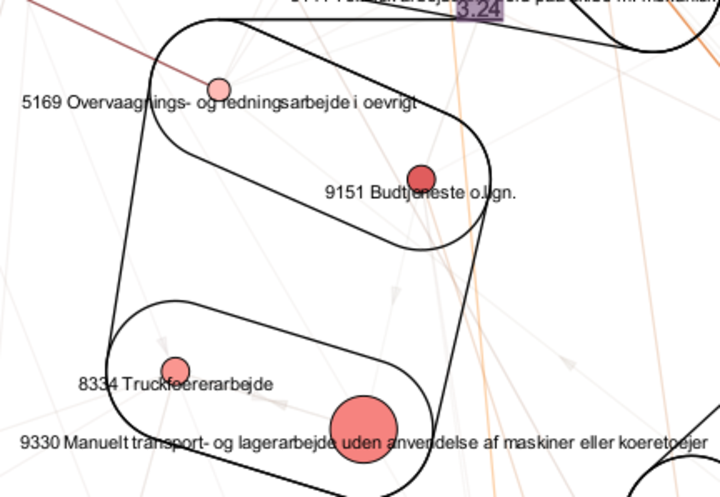
\includegraphics[width=6cm]{fig/segzoom/seg_3_24.pdf}
   \caption{}
   \label{fig_delanalyse1_zoom_3_24}
  \end{center}
  \vspace{-20pt}
\end{wrapfigure}
%

Set ud fra Goldthorpes syn på arbejdskontrakter, er det jobs, hvor specifiteten af af kompetencer er lav, og muligheden for overvågning af arbejdet må antages at være høj. Det er desuden hårdt fysisk arbejde, eller, i  texttt{5169}'s tilfælde, arbejde, der kræver en god fysisk form. Det er ikke overraskende, at denne type arbejde har en høj frafaldsprocent. % men hvor frafalder den hen? \#todo      

For de fleste klynger er den interne mobilitet højere end 70 \%. Få klynger som dem der bl.a. er blevet beskrevet ovenfå har en internmobilitet på helt ned til 50 \%. Fælles for klyngerne er, at de vurderes til at være afgrænset i sådan et omfang, at der er væsentlige barrierer mellem klynget og resten af arbejdsmarkedet, der gør, at der inden for klynget er en nærhed, hvor mobilitet er “let og typisk”.


%%%%%%%%%%%%%%%%%%%%%%%%%%%%%%%%%%%%%%%%%%%%%%
\section{Delkonklusion \label{}}
%%%%%%%%%%%%%%%%%%%%%%%%%%%%%%%%%%%%%%%%%%%%%%

Formålet med dette kapitel har været at besvare forskningspørgsmålet: Er der en opdeling af arbejdsmarkedet for arbejdstagere i delmarkeder, hvor mobilitet indenfor delmarkederne er hyppig, og mellem delmarkederne sjælden?

Moneca-algoritmen har aggreret 273 jobfunktioner til 51 klynger. Denne opdeling afspejler Boje (1986) og Toubøl (2913). Klyngedannelsen er skabt via Moneca-algoritment og kvalitetsvurderet fra niveau til niveau. Der er i alt blevet splittet fire klynger op, som ud fra mobilitet, densitet og antal stier ikke har kunne vurderes som meningsfulde delmarkeder. 79 \% af al mobilitet foregår inden for delmarkeder, det vil sige, at mobilitet indenfor delmarkederne er hyppig, og mellem delmarkederne sjælden. Klyngerne skabt i aggreringen kan derfor betragtes som delmarkeder.